\documentclass[9pt,a4paper,twocolumn,twoside]{tau-class/tau}
\usepackage[spanish,es-nodecimaldot,es-noindentfirst]{babel}

\doctype{Reporte Ejecutivo Integrado}
\title{Reporte de performance y panorama competitivo: Centro de Psicologia Integral y Terapia - Psicotelcon}

\author[a,1]{Equipo de Analitica Oderbiz}
\affil[a]{Unidad de Inteligencia Comercial}

\dates{Compilado el \today}
\docinfo{Documento generado con datos internos en formato \texttt{llm\_context\_report.page.v1}, investigacion competitiva publica y evidencia visual automatizada. Toda lectura no directamente observable se etiqueta como \texttt{inferencia}.}
\footinfo{Reporte Oderbiz}
\theday{\today}
\organization{Oderbiz}
\leadauthor{Equipo Oderbiz}

\begin{abstract}
En la ventana \texttt{last\_30d}, la cuenta analizada invirtio \$21.30 y alcanzo 14{,}759 impresiones con 12{,}695 de alcance (\texttt{observado}). El rendimiento de atencion inicial es positivo (CTR 1.57\% y 209 clics unicos), con conversion conversacional de 11 conversaciones iniciadas y 11 primeras respuestas (\texttt{observado}). Sin embargo, la calidad de trafico muestra dependencia total de mensajeria dentro de plataforma al no registrar outbound clicks (\texttt{observado}). El entorno competitivo local presenta alta fragmentacion entre perfiles individuales, centros integrales y directorios comparativos (\texttt{observado}). La prioridad estrategica es fortalecer diferenciacion por problema clinico, estandarizar arquitectura de campanas y medir calidad post-conversacion para mejorar eficiencia de crecimiento (\texttt{inferencia}).
\end{abstract}

\keywords{Meta Ads, psicologia, Loja, mensajeria, inteligencia competitiva}

\begin{document}
\maketitle
\thispagestyle{firststyle}

\section{Resumen ejecutivo}

La operacion paid actual genera volumen eficiente en alcance y clics con baja inversion absoluta (\texttt{observado}). El cuello de botella principal no es la captacion de atencion, sino la trazabilidad de negocio posterior al primer contacto (\texttt{inferencia}). En geo, Loja concentra casi todo el resultado (10 de 11 conexiones de mensajeria), con Zamora Chinchipe como extension secundaria (\texttt{observado}). En demografia, 25--44 concentra volumen; 55+ aporta señales de CTR/CPC favorables a menor escala (\texttt{observado}+\texttt{inferencia}).

\section{Contexto del negocio y periodo analizado}

\begin{itemize}
  \item Nombre de pagina: \texttt{Centro de Psicologia Integral y Terapia - Psicotelcon}
  \item ID de pagina: \texttt{1506380769434870}
  \item Nombre de cuenta: \texttt{Dra Marizol Jimenez Luzon}
  \item ID de cuenta: \texttt{act\_131112367482947}
  \item Campana filtrada: \texttt{N/A} (sin filtro aplicado)
  \item ID campana filtrada: \texttt{N/A}
  \item Moneda: \texttt{USD}
  \item Zona horaria: \texttt{America/Guayaquil}
  \item Rango analizado: \texttt{last\_30d}
\end{itemize}

\section{Baseline interno}

\subsection{KPIs base}
\begin{itemize}
  \item Inversion: \$21.30; impresiones: 14{,}759; alcance: 12{,}695 (\texttt{observado}).
  \item CTR: 1.565\%; CPM: \$1.44 (\texttt{observado}).
  \item Embudo: 209 clics unicos; 11 conversaciones iniciadas; 11 primeras respuestas (\texttt{observado}).
  \item Calidad de trafico: 0 outbound clicks; costo por clic unico: \$0.10 (\texttt{observado}).
\end{itemize}

\subsection{Tendencia temporal}
Los dias de mayor entrega (25-mar, 20-abr, 21-abr) sostienen CTR entre 1.56\% y 1.88\%, con CPM entre 1.19 y 1.67 (\texttt{observado}). Esto describe una operacion estable a pequena escala pero sensible a subasta al aumentar ritmo de entrega (\texttt{inferencia}).

\subsection{Embudo y calidad}
La relacion 209 clics unicos vs 11 conversaciones iniciadas implica una tasa aproximada de 5.3\% de clic unico a conversacion (\texttt{estimado}). La ausencia de outbound clicks confirma dependencia de interaccion in-platform y baja visibilidad de conversion fuera de Meta (\texttt{observado}+\texttt{inferencia}).

\subsection{Senal geo y demografica}
Loja concentra 96.4\% del gasto (20.53/21.30) y 10/11 resultados de mensajeria; Zamora Chinchipe aporta escala marginal con CPA menor sobre muestra pequena (\texttt{observado}+\texttt{inferencia}).

Por edad, los rangos 25--44 concentran volumen y resultados; 55--64 y 65+ muestran senales de CPC eficiente para pruebas de escala controlada (\texttt{observado}+\texttt{inferencia}).

\section{Panorama competitivo}

El mercado local combina tres capas: perfiles individuales con especialidad, centros con oferta integral y directorios que facilitan comparacion rapida por ciudad/servicio (\texttt{observado}). La implicacion estrategica es diferenciar mensajes por resultado terapeutico y no solo por disponibilidad (\texttt{inferencia}).

\subsection{Evidencia visual competitiva}

\begin{figure}[H]
  \centering
  
\includegraphics[width=0.95\columnwidth]{figures/centro-de-psicologia-integral-y-terapia-psicotelcon/fig-panorama-psicologiaymente-marizol-20260425-v1.png}
  \caption{Perfil profesional en directorio especializado (evidencia de posicionamiento y especialidad).}
  \label{fig:competencia_psicologiaymente}
\end{figure}
\textbf{Fuente:} \url{https://psicologiaymente.com/psicologos/2069561/dra-marizol-jimenez-luzon} (captura: 2026-04-25T12:03:00-05:00).

\begin{figure}[H]
  \centering
  
\includegraphics[width=0.95\columnwidth]{figures/centro-de-psicologia-integral-y-terapia-psicotelcon/fig-panorama-psicoorg-directorio-loja-20260425-v1.png}
  \caption{Directorio local por ciudad y especialidad (evidencia de comparabilidad competitiva).}
  \label{fig:competencia_psicoorg}
\end{figure}
\textbf{Fuente:} \url{https://www.psico.org/ec/directorio/loja} (captura: 2026-04-25T12:04:00-05:00).

\begin{figure}[H]
  \centering
  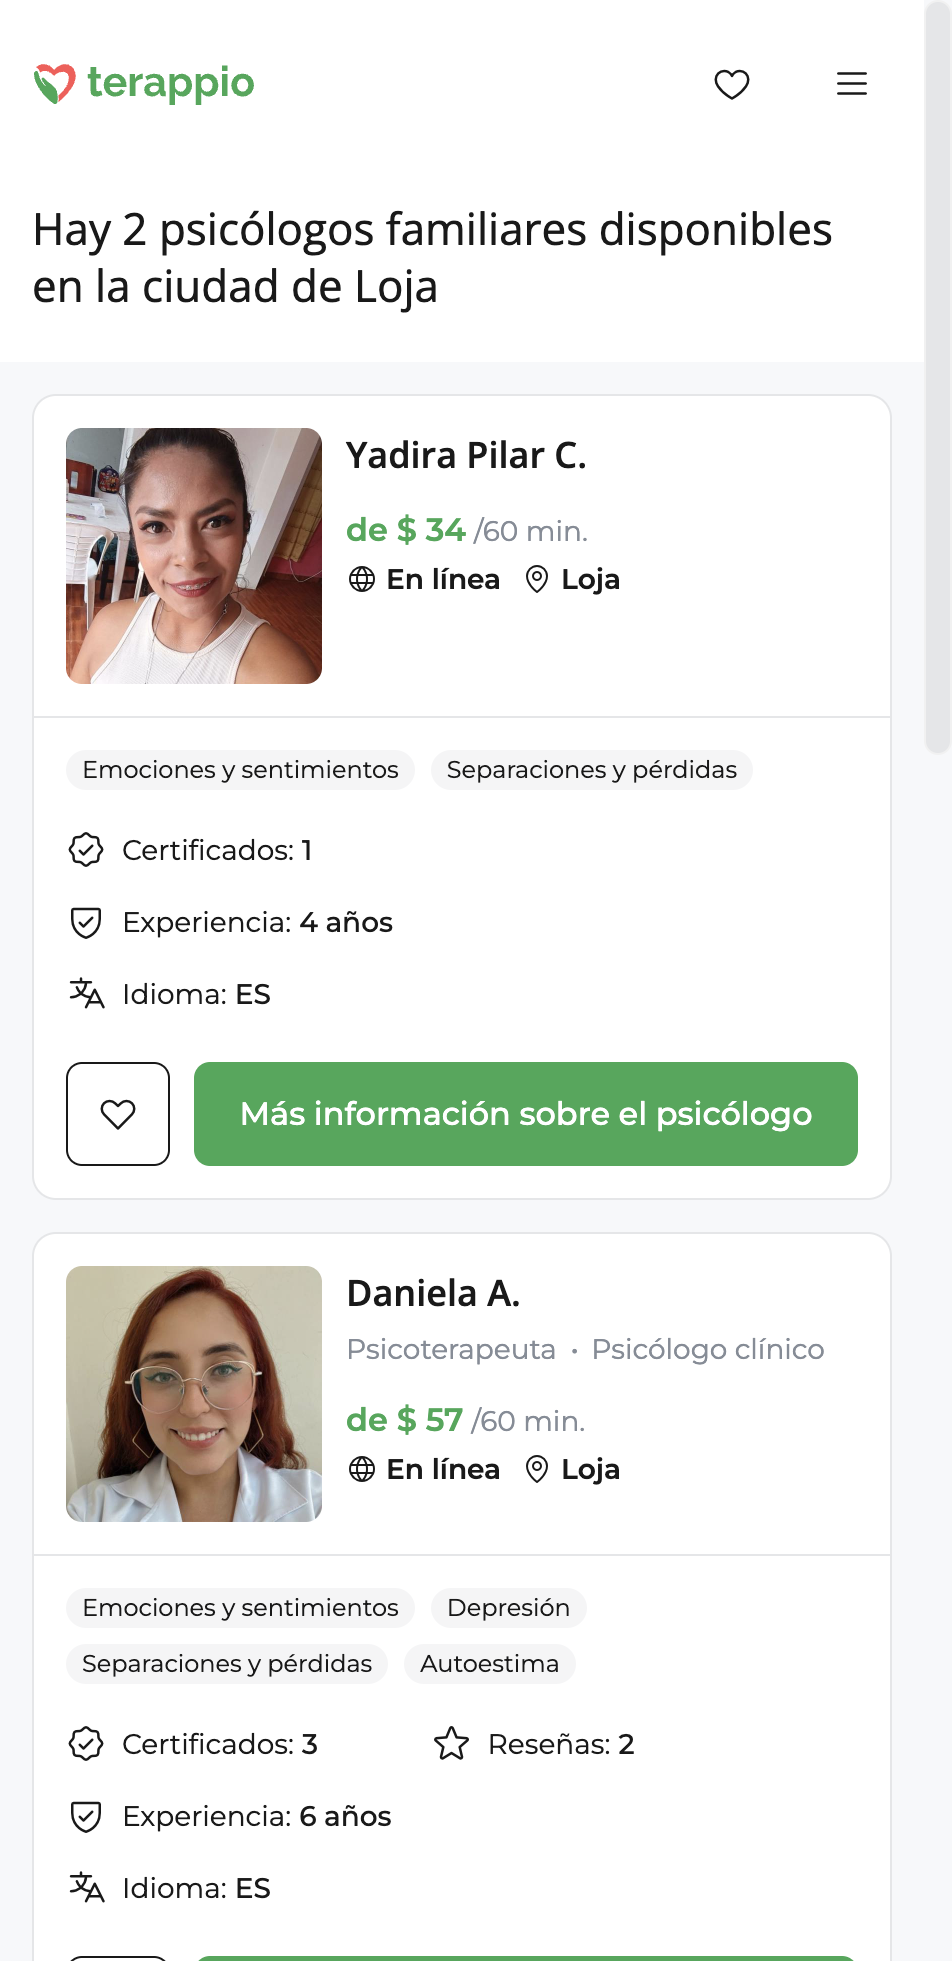
\includegraphics[width=0.95\columnwidth]{figures/centro-de-psicologia-integral-y-terapia-psicotelcon/fig-panorama-terappio-loja-20260425-v1.png}
  \caption{Marketplace con oferta de terapeutas en Loja (evidencia de referencia de precio y propuesta).}
  \label{fig:competencia_terappio}
\end{figure}
\textbf{Fuente:} \url{https://www.terappio.com/ec/family-therapist/ecuador/loja} (captura: 2026-04-25T12:05:00-05:00).

\section{Diagnostico integrado}

\subsection{Fortalezas}
\begin{itemize}
  \item Cobertura eficiente con baja inversion absoluta (\texttt{observado}).
  \item Capacidad consistente para iniciar y sostener conversacion (\texttt{observado}).
  \item Continuidad operativa y base amplia de campanas historicas (\texttt{observado}).
\end{itemize}

\subsection{Brechas}
\begin{itemize}
  \item Cero salida outbound y baja atribucion fuera de Meta (\texttt{observado}).
  \item Nomenclatura heterogenea de campanas dificulta aprendizaje analitico (\texttt{observado}).
  \item Sin cierre CRM en el JSON (citas atendidas/ticket), limita lectura de impacto economico (\texttt{observado}).
\end{itemize}

\subsection{Riesgos}
\begin{itemize}
  \item Dependencia de un solo canal de conversacion (\texttt{inferencia}).
  \item Exposicion a comparacion de oferta/precio en directorios y marketplaces (\texttt{observado}).
  \item Sensibilidad de costos ante escalamiento de entrega diaria (\texttt{inferencia}).
\end{itemize}

\subsection{Oportunidades}
\begin{itemize}
  \item Creatividades por motivo de consulta (lenguaje, conducta, desarrollo, familia) (\texttt{inferencia}).
  \item Embudo dual \texttt{MESSAGES + TRAFFIC} para elevar trazabilidad de negocio (\texttt{inferencia}).
  \item Expansion geo controlada usando senales de CPA por provincia (\texttt{inferencia}).
\end{itemize}

\section{Plan de accion priorizado}

\subsection{P1 (alto impacto / bajo esfuerzo)}
\begin{itemize}
  \item Estandarizar naming de campanas: objetivo--audiencia--oferta--fecha.
  \item Crear tablero semanal: costo por conversacion iniciada, primera respuesta y cita agendada.
  \item Lanzar 3 variantes de copy por dolor clinico.
  \item Protocolo de respuesta inicial para reducir tiempo de atencion.
\end{itemize}

\subsection{P2 (alto impacto / esfuerzo medio-alto)}
\begin{itemize}
  \item Activar campana complementaria de trafico con landing de conversion.
  \item Implementar taxonomia de audiencias por necesidad terapeutica.
  \item Test quincenal por formato creativo (testimonio, educativo, caso).
  \item Instrumentar calidad post-chat (contacto efectivo, asistencia, continuidad).
\end{itemize}

\subsection{P3 (experimental)}
\begin{itemize}
  \item Lookalikes de conversaciones de alta calidad.
  \item Retargeting por profundidad conversacional.
  \item Alianzas de contenido con actores locales de salud/educacion.
\end{itemize}

\section{Fuentes y limitaciones}

\subsection{Fuentes internas}
\begin{itemize}
  \item \texttt{report\_metadata}, \texttt{page\_overview}, \texttt{timeseries\_daily}
  \item \texttt{funnel}, \texttt{traffic\_quality}
  \item \texttt{geo}, \texttt{demographics}
  \item \texttt{campaigns\_available}, \texttt{reference\_link\_coverage}, \texttt{module\_status}
\end{itemize}

\subsection{Fuentes competitivas y visuales}
\begin{itemize}
  \item \url{https://psicologiaymente.com/psicologos/2069561/dra-marizol-jimenez-luzon}
  \item \url{https://www.psico.org/ec/directorio/loja}
  \item \url{https://www.terappio.com/ec/family-therapist/ecuador/loja}
  \item \url{https://tecnologicosudamericano.edu.ec/bienestar-estudiantil/centro-psicoterapeutico-la-cabana/}
  \item \url{https://facebook.com/PsicotelconTerapias}
\end{itemize}

Las rutas locales de evidencia visual y metadatos de captura se registran en:
\texttt{docs/reports/figures/centro-de-psicologia-integral-y-terapia-psicotelcon/CAPTURAS.md}

\subsection{Limitaciones}
\begin{itemize}
  \item No se ejecuto \texttt{apify-market-research} por falta de confirmacion de token/creditos.
  \item El activo de Facebook presenta vista de acceso/login; evidencia valida de presencia publica pero con detalle parcial de contenido.
  \item No hay datos CRM de cierre en el JSON, por lo que el impacto en revenue queda parcial.
\end{itemize}

\end{document}
